\clearpage
\section{石柱的表面与光照}
神庙的石柱底色很浅，背光的一面却是深灰。要算出这层差别，先得知道镜头看见的是哪块石头，再查它的颜色和朝向。三角形投影到屏幕后，覆盖的采样位置会产生片元，这一步叫光栅化。深度测试留下最近、也通过材质透明度裁剪的一层。

\begin{figure}[H]\centering
\begin{minipage}[t]{.483\linewidth}\centering
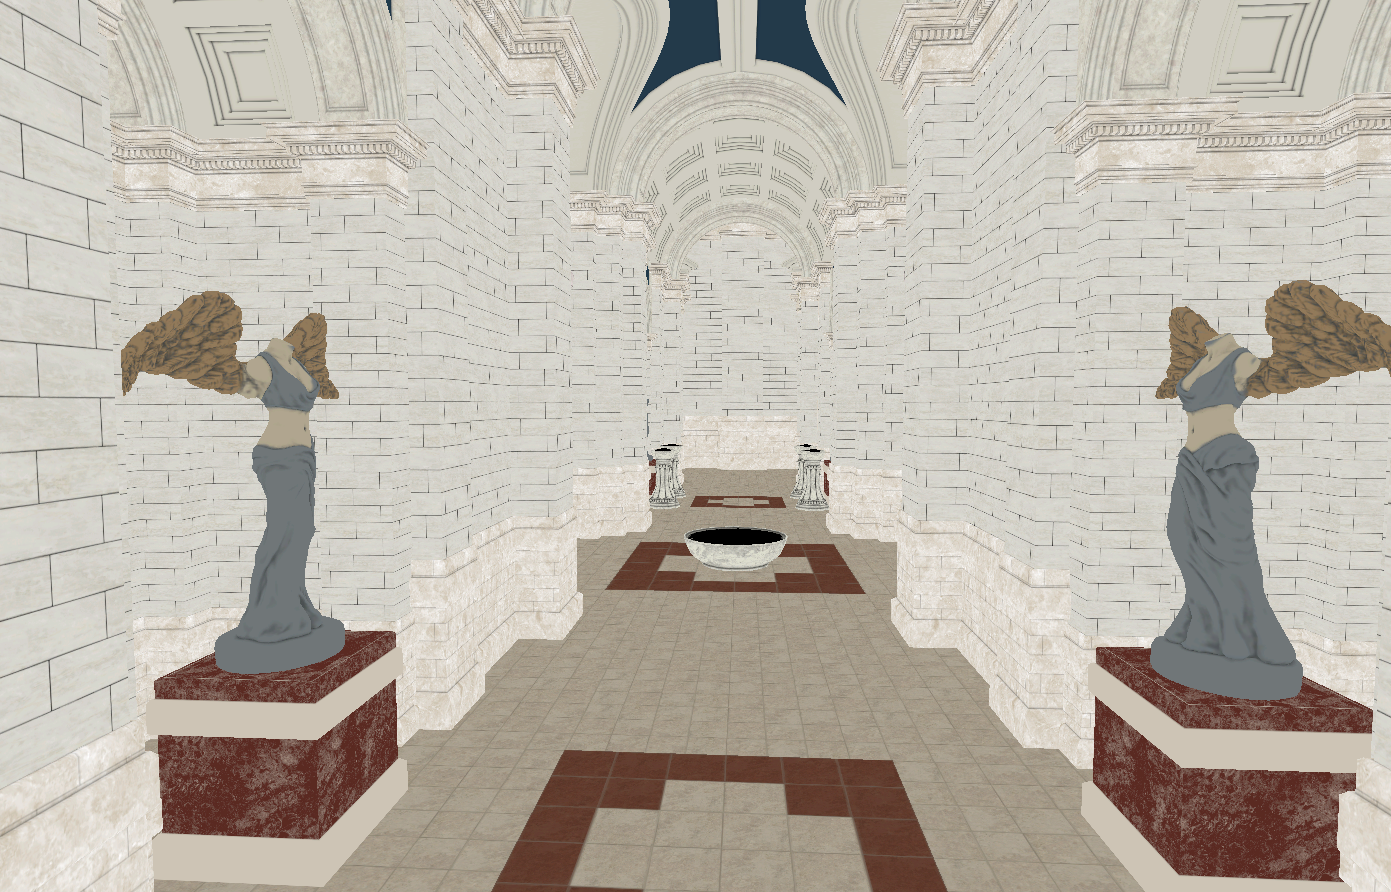
\includegraphics[width=\linewidth]{../../../output/scenes/sun-temple/albedo.png}\\
{\sffamily\small 材质的底色}
\end{minipage}\hfill
\begin{minipage}[t]{.483\linewidth}\centering
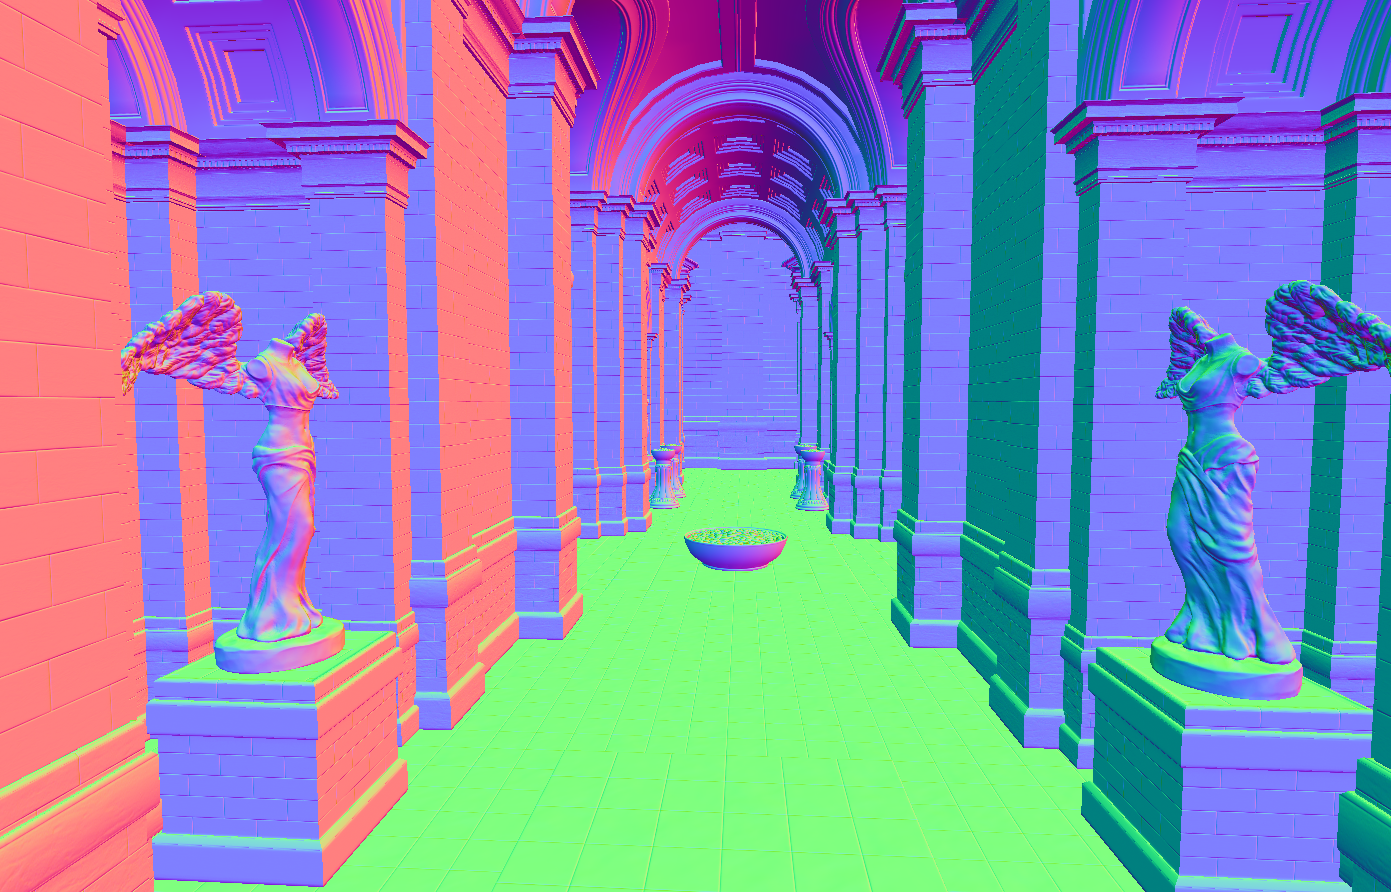
\includegraphics[width=\linewidth]{../../../output/scenes/sun-temple/normal-depth.png}\\
{\sffamily\small 世界坐标中的法线}
\end{minipage}
\caption{同一次绘制的两个输出。左图的石块之间只有细微色差；在右图，面向镜头的墙接近蓝色、向上的地面是绿色，墙上斜切的线脚又有其他颜色。右图以 RGB 标出法线的 $x,y,z$ 三个分量，深度在第四个分量中。}
\end{figure}

\begin{figure}[H]\centering
\begin{tikzpicture}[x=1mm,y=1mm,every node/.style={font=\sffamily\small,text=Ink},
    station/.style={draw=Rule,rounded corners=1.2mm,align=center,inner sep=2.4mm},
    arrow/.style={-{Stealth[length=2mm]},draw=Teal,line width=.75pt}]
  \draw[draw=Rule,rounded corners=1.4mm] (0,0) rectangle (155,34);
  \node[station,fill=Soft] (raster) at (25,17) {\texttt{Mesh.frag}\\底色、法线与深度};
  \node[station,fill=warm] (pack) at (79,17) {\texttt{PackSurfaces.comp}\\还原每个位置};
  \node[station,fill=pale] (lit) at (134,17) {\texttt{RenderLit}\\直接光与间接光};
  \draw[arrow] (raster)--(pack);
  \draw[arrow] (pack)--(lit);
\end{tikzpicture}
\caption{箭头沿着显存中的数据走。左段读取同一帧的两张图，中段写入包含位置、法线和底色的 \code{GISurface} 数组，右段按像素使用它。}
\end{figure}

从相机看到的深度仍是投影之后的数。比如图像正中的石壁，深度是 $0.99738$。要照亮它，还需要知道它离场景中的点光源有多远。\code{PackSurfaces.comp} 取出这个深度，按 $2d-1$ 换回引擎相机使用的范围，与像素中心的横、纵坐标组成四维向量。乘以本次相机矩阵的逆，再除以结果的 $w$，得到石壁在世界中的位置。这次投影若有 TAA 的采样偏移，还原时也使用同一次偏移。

镜头看见的第一层由光栅绘制取得。计算阴影和间接光时，着色器还要查询离开这一层的光线会撞上哪个三角形。两段工作通过显存交换数据，当前实现会等待每段提交完成。图中模型为 Epic Games 的 Sun Temple，项目的布光与衍生截图沿用 CC BY-NC-SA 4.0 许可。

\readings{\src{Redflag/src/Platform/Vulkan/Shaders/Mesh.frag}{Mesh.frag}\quad
\src{Redflag/src/Platform/Vulkan/Shaders/PackSurfaces.comp}{PackSurfaces.comp}\quad
\href{run:../scenes/sun-temple/capture.json}{RenderDoc 帧与像素}\quad
\href{https://developer.nvidia.com/ue4-sun-temple}{NVIDIA ORCA 原场景}\\
\href{https://www.cs.cornell.edu/courses/cs4620/2018fa/slides/10rasterization.pdf}{虎书作者 Marschner · 光栅化讲义，第 3 页}}
